\documentclass[11pt,letterpaper]{article}

%\usepackage{fontspec}
%\usepackage[utf8]{inputenc}
\usepackage{textcomp,marvosym}
\usepackage{amsmath,amssymb}
\usepackage[normalem]{ulem}
\usepackage[left]{lineno}
\usepackage{changepage}
\usepackage{rotating}
\usepackage{color}
\usepackage{natbib}
\usepackage{setspace}
\usepackage{}
\usepackage{fancyhdr}
\usepackage{graphicx}
\usepackage{xspace}
\usepackage{threeparttable}
\usepackage{color,colortbl}
\usepackage{url}
%\usepackage[hidelinks]{hyperref}
\urlstyle{same}
\doublespacing

\raggedright
\textwidth = 6.5 in
\textheight = 8.25 in
\oddsidemargin = 0.0 in
\evensidemargin = 0.0 in
\topmargin = 0.0 in
\headheight = 0.0 in
\headsep = 0.5 in
\parskip = 0.1 in
\parindent = 0.1in

% Bold the 'Figure #' in the caption and separate it from the title/caption with a period
% Captions will be left justified
\usepackage[aboveskip=1pt,labelfont=bf,labelsep=period,justification=raggedright,singlelinecheck=off]{caption}

% Remove brackets from numbering in List of References
%\makeatletter
%\renewcommand{\@biblabel}[1]{\quad#1.}
%\makeatother

% Self defined commands
\newcommand{\degC}{$^{\circ}$C\xspace}
\newcommand{\dC}{$\delta^{13}$C\xspace}
\newcommand{\dO}{$\delta^{18}$O\xspace}
\newcommand{\SrSr}{$^{87}$Sr/$^{86}$Sr\xspace}
\newcommand{\permil}{\textperthousand\xspace}
\newcommand{\dsil}{$d$\xspace}

\setcounter{figure}{0}
\renewcommand{\thefigure}{DR\arabic{figure}}
\setcounter{table}{0}
\renewcommand{\thetable}{DR\arabic{table}}

\definecolor{Yellow}{rgb}{1,1,0.35}
%

\pagestyle{myheadings}
\pagestyle{fancy}
\fancyhf{}
\lhead{Park et al., in preparation for GSA Bulletin}
\rhead{\thepage}

\begin{document}

\begin{flushleft}
{\Large \textbf{Data Repository for ``The lead-up to the Sturtian Snowball Earth: Neoproterozoic chemostratigraphy time-calibrated by the Tambien Group of Ethiopia''}}
\\
Yuem Park\textsuperscript{1},
Nicholas L. Swanson-Hysell\textsuperscript{1},
Scott A. MacLennan\textsuperscript{2},
Adam C. Maloof\textsuperscript{2},
Mulubrhan Gebreslassie\textsuperscript{3,4},
Marissa M. Tremblay\textsuperscript{1,5},
Blair Schoene\textsuperscript{2},
Mulugeta Alene\textsuperscript{3},
Eliel S. C. Anttila\textsuperscript{1,6},
Tadele Tesema\textsuperscript{3},
Bereket Haileab\textsuperscript{7}
\\
\bigskip
\textsuperscript{1} Department of Earth and Planetary Science, University of California, Berkeley, CA, USA
\\
\textsuperscript{2} Department of Geosciences, Princeton University, Princeton, NJ, USA
\\
\textsuperscript{3} School of Earth Sciences, Addis Ababa University, Addis Ababa, Ethiopia
\\
\textsuperscript{4} Current affiliation: Department of Applied Geology, Adama Science and Technology University, Adama, Ethiopia
\\
\textsuperscript{5} Current affiliation: Scottish Universities Environmental Research Centre, East Kilbride, Scotland, UK
\\
\textsuperscript{6} Current affiliation: Department of Earth and Planetary Science, Harvard University, Cambridge, MA, USA
\\
\textsuperscript{7} Department of Geology, Carleton College, Northfield, MN, USA
\bigskip

\end{flushleft}

\linenumbers

This document accompanies the discussion contained in the main text. All the Python code used for this study, as well as the associated data tables not included in this document, can be found at: \url{https://github.com/Swanson-Hysell-Group/2018_Tambien_Group}.

\clearpage

\section*{Construction of the Chemostratigraphic Composite}

The main text contains a composite \dC and \SrSr curves for the Tonian and Cryogenian that are time-calibrated by the record from Ethiopia and incorporate data from the literature from numerous sources. Additional details associated with the data sets within this composite are provided below. The Python code used to develop the composite as well as the associated data table can be found at: \url{https://github.com/Swanson-Hysell-Group/2018_Tambien_Group}.

\subsubsection*{Ethiopia}

\dC and \SrSr data from Ethiopia comes from the Tambien Group and are developed in \citet{Miller2009a}, \citet{Swanson-Hysell2015a}, and this study. Combined with U-Pb ID-TIMS dates on zircons from \citet{Swanson-Hysell2015a} (815.29$\pm$0.32, 788.72$\pm$0.24, and 787.38$\pm$0.14~Ma) and new U-Pb ID-TIMS dates on zircons from \citet{MacLennan2018a} (735.25$\pm$0.25, 719.58$\pm$0.56, and 719.68$\pm$0.46~Ma), the Tambien Group is now the source of the most temporally well-constrained pre-Sturtian chemostratigraphic dataset to date. We therefore use the Tambien Group \dC curve as the backbone for making correlations with other datasets. In the chemostratigraphic composite, the age of the initiation of the Sturtian Glaciation is set to 717~Ma (discussed further in the `Onset of the Sturtian Snowball' section).

\subsubsection*{Svalbard}

\dC and \SrSr data from Svalbard come from the Akademikerbreen Group and are developed in \citet{Halverson2007b} and \citet{Halverson2007a}. However, a slightly stricter threshold for \SrSr diagenesis is applied to the data included in our composite than in the original publication ([Sr]\textless500~ppm). Additional \SrSr data were published in \citet{Cox2016a}. The Polarisbreen Group, which unconformably overlies the Akademikerbreen Group, contains two separate diamictite units which have been interpreted to represent the Sturtian and Marinoan Glaciations respectively \citep{Halverson2004a}. This correlation constrains the Akademikerbreen Group to have been deposited prior to the Sturtian Glaciation. No direct geochronological constraints exist for the Akademikerbreen Group although thermal subsidence models have been used to suggest a ca. 800~Ma age for the Bitter Springs Stage \citep{Maloof2006a}. Therefore, the \dC curve from the group is correlated to that of the Tambien Group by aligning the start and end of the Bitter Springs Stage and the nadir of the Islay Anomaly. This correlation results in a near constant sedimentation rate between these constraints, which is used to estimate the age of data that precedes the Bitter Springs Stage.

\subsubsection*{Greenland}

\dC and \SrSr data from the Eleanore Bay Supergroup are developed in \citet{Cox2016a}. \citet{Halverson2004a} approximated the age of the this succession to be ca. 800~Ma based on the correlation of lithological and \dC data to the Akademikerbreen Group of Svalbard, but no direct age constraints exist. Therefore, the age model is estimated based on aligning the \dC data with the \dC curve of the Akademikerbreen Group.

\subsubsection*{Australia}

\dC data from the Bitter Springs Formation are developed in \citet{Swanson-Hysell2010a}. Further \SrSr data are developed in \citet{Cox2016a}. Similar to the Akademikerbreen Group, the Bitter Springs Formation is unconformably overlain by Sturtian diamictite of the Areyonga Formation \citep{Swanson-Hysell2010a}, and thus constrains the Bitter Springs Formation to have been deposited prior to the Sturtian Glaciation. However, no direct geochronological constraints exist for the Bitter Springs Formation. Therefore, the \dC curve from this group is correlated to that of the Tambien Group by aligning the start and end of the Bitter Springs Stage. Again, this correlation results in a near constant sedimentation rate between these constraints, which is used to estimate the age of data that post-dates the Bitter Springs Stage. However, if the constant sedimentation rate is applied to \dC data from the Bitter Springs Formation preceding the Bitter Springs Stage, there is a significant mismatch between these data and that of the Akademikerbreen Group. Therefore, these data were assigned slightly older ages than would be predicted by the constant sedimentation rate assumption in order to better match the \dC curves between these two sections.

\subsubsection*{Canada}

\dC and \SrSr data from Canada come from multiple studies and localities.

\dC data and geochronology from the Fifteenmile Group are developed in \citet{Macdonald2010a}. Additional \SrSr data are developed in \citet{Cox2016a}. The Fifteenmile Group is unconformably overlain by temporally well-constrained (see the `Onset of the Sturtian Snowball' section) Sturtian diamictite of the Upper Mount Harper Group \citep{Macdonald2010a}. A U-Pb ID-TIMS date on zircons within a tuff of 811.51$\pm$0.25~Ma can be tied directly to this curve, and, combined with dates from the Tambien Group (787.38$\pm$0.14, 788.72$\pm$0.24, and 815.29$\pm$0.32~Ma), suggests global synchroneity of the Bitter Springs Stage \citep{Swanson-Hysell2015a}. The nadir of the Islay Anomaly can also be easily identified and correlated. Furthermore, \dC data that precede the Bitter Springs Stage correlate well with data from the Akademikerbeen Group, and thus were correlated based on similar \dC values. However, unlike other sections in which the Bitter Springs Stage is observed, the recovery from the interval of low \dC values appears to be much more gradual. Nevertheless, the end of the minimum \dC values is assumed to be correlative to the end of the Bitter Springs Stage, and a roughly constant sedimentation rate was applied to the data between this age and the Islay Anomaly nadir, excluding an unconformity interpreted to exist between PF1 and PF3 of the Fifteenmile Group \citep{Macdonald2010a}.

\dC and \SrSr data from the Little Dal Group are developed in \citet{Halverson2006a} and \citet{Halverson2007b}. A slightly stricter threshold for \SrSr diagenesis is applied to the data included in our composite ([Sr]\textless250~ppm and Mn/Sr\textgreater0.15) than in the original work. A basalt has been interpreted to conformably overlie the Little Dal Group \citep{Aitken1981a} and inferred to have erupted ca. 780~Ma based on geochemical similarity to mafic dikes and sills that intrude the Mackenzie Mountain Supergroup \citep{Harlan2003a}. Given that the basalt has not been directly dated, there is some uncertainty associated with this interpretation. Nevertheless, correlating the \dC curve from the Little Dal Group to that of the Tambien Group by aligning the start and end of the Bitter Springs Stage and assuming constant sedimentation rate throughout the rest of the section suggests that the top of the Little Dal Group is ca. 780~Ma, consistent with the inference of \citet{Harlan2003a}.

\dC and \SrSr data and geochronology from the Coates Lake Group are developed in \citet{Halverson2006a}, \citet{Halverson2007b}, and \citet{Rooney2014a}. A Re-Os isochron date on black shales of 732.2$\pm$3.9~Ma can be tied directly to this curve as it comes from strata recording the recovery from the nadir of the Islay \dC Anomaly. This date provides constraints on the temporal alignment of the curve. Given the uncertainty associated with the date, the correlation is further refined by aligning the nadir and recovery of the excursion with the Tambien Group data.

\dC and \SrSr data from the Shaler Supergroup are developed in \citet{Asmerom1991a}, although \SrSr data with Mn/Sr\textgreater3 and \dO\textless-10\permil are considered to be altered. Further \dC data are developed in \citet{Jones2010a}. Age constraints on these strata are poor. However, the onset of the Bitter Springs Anomaly and the Islay Anomaly as well as other minor inflexions in the \dC curve are identifiable in the data. Furthermore, lithostratigraphic correlations between the Shaler Supergroup and the Mackenzie Mountains Supergroup can be made. Therefore, the age model for these data is developed based on the correlation of the \dC curve as well as the lithostratigraphy between these two supergroups, as in \citet{Jones2010a}.

\subsubsection*{Scotland}

\dC and \SrSr data from the Dalradian Supergroup are developed in \citet{Sawaki2010a}. The carbonates from which these data are sourced unconformably underlie a glacial diamictite. \citet{Brasier2000a} argues that \SrSr values from these carbonates are too low (\textless0.7065) to be post-Sturtian, and therefore must be pre-Sturtian in age. Besides this argument, no direct geochronological constraints exist for the Dalradian Supergroup. Therefore, the \dC curve from this group is correlated to that of the Tambien Group by aligning the nadir of the Islay Anomaly.

\subsubsection*{Russia}

\dC and \SrSr data from Siberia come from multiple sources.

\dC and \SrSr data from the Proterozoic carbonates of the Uchur–Maya and Turukhansk regions of Siberia are developed in \citet{Bartley2001a}, with additional \SrSr data from \citet{Cox2016a}. All available \SrSr data from \citet{Bartley2001a} had [Sr]\textless500~ppm, and as a result Mn/Sr\textgreater0.5 is the only threshold applied for diagenesis. Age constraints on these strata are poor. Therefore, the age model applied to these data was based on lithostratigraphic correlation to the Yenisey Ridge and Uchur Maya Region sections, which are temporally constrained to have been deposited ca. 1100-1000~Ma based on geochronological constraints of varying robustness \citep{Gallet2012a}.

\dC and \SrSr data from the Karatau Group of the Urals are developed in \citet{Kuznetsov2006a}, with additional \SrSr data from \citep{Cox2016a}. However, a slightly stricter threshold for \SrSr diagenesis was applied to the data included in our composite ([Sr]\textless350~ppm and Mn/Sr\textgreater0.1). Correlation of microbiota across Siberia suggests that the group is younger than ca. 1030~Ma \citep{Kuznetsov2006a}. However, no other direct age control is available for this group. Therefore, following \citet{Cox2016a}, the age model for the Karatau Group data is constructed based on the correlation of one ca. 970~Ma Turukhansk Uplift \SrSr measurement to the start of the Karatau Group data.

\subsection*{Cryogenian Successions}

Since Tambien Group chemostratigraphy is limited to the Tonian, our Cryogenian \dC and \SrSr chemostratigraphic composite is a compilation of a number of other Cryogenian datasets. In general, correlations between datasets are made using absolute age constraints where possible - otherwise, characteristic negative \dC excursions (the ca. 659~Ma Rasthof Excursion, the ca. 655~Ma Taishir Anomaly, and the ca. 643~Ma Trezona Anomaly) are used to align datasets. Unless mentioned otherwise, the same criteria for diagenesis that were used for publication of the original datasets are applied here.

\subsubsection*{Mongolia}

\dC and \SrSr data from Mongolia come from the Tsagaan-Olam Group and are developed in \citet{Bold2016a} and \citet{Brasier1996a}. Given that data from this group span the entirety of the Cryogenian and into the Ediacaran, we use it as the backbone for our Cryogenian composite. For both datasets we apply a [Sr]\textless500~ppm and Mn/Sr\textgreater0.3 threshold for \SrSr diagenesis.

The age model for these data follows that of \citet{Bold2016a}. A minimum age for the end of the Sturtian Glaciation is constrained by the following: U-Pb ID-TIMS on zircon from a tuffaceous bed overlying Sturtian diamicite in south China yields an age of 662.9$\pm$4.3~Ma \citep{Zhou2004a}, a Re-Os isochron on black shales overlying Sturtian diamictite in northwest Canada yields an age of 662.4$\pm$4.6~Ma \citep{Rooney2014a}, and a Re-Os isochron on black shales overlying Sturtian diamictite in Mongolia yields an age of 659.0$\pm$4.5~Ma \citep{Rooney2015a}. A maximum age for the end of the Sturtian Glaciation is constrained by U-Pb ID-TIMS on zircon from a tuff interbedded with Sturtian diamictite in Australia, which yields an age of 663.03$\pm$0.11~Ma \citep{Cox2018b}. Therefore, for our Cryogenian composite, we set the age of the end of the Sturtian Glaciation (and therefore the age of the base of the Tsagaan-Olam Group) to 660~Ma.

A maximum age for the start of the Marinoan Glaciation comes from a U-Pb SHRIMP age on zircon from a tuff underlying Marinoan diamictite in south China of 654.5$\pm$3.8~Ma \citep{Zhang2008b}. However, this tuff is separated from the Marinoan diamictite by a major disconformity, and so the age for the start of the Marinoan Glaciation is likely significantly younger than this U-Pb SHRIMP age. Therefore, following \citet{Bold2016a}, we set the age for the start of the Marinoan Glaciation in our composite to be 640~Ma.

The end of the Marinoan Glaciation is tightly temporally constrained. Zircons from a volcanic ash within and just above Marinoan diamictite in south China yielded U-Pb ID-TIMS dates of 635.5$\pm$0.6 and 635.2$\pm$0.6~Ma respectively \citep{Condon2005a}. This constraint is consistent with U-Pb ID-TIMS dates from zircon from tuffs within Marinoan diamictite of 635.5$\pm$1.2~Ma in Namibia \citep{Hoffmann2004a}, and 636.4$\pm$0.5~Ma in Tasmania, Australia \citep{Calver2013a}.

\subsubsection*{Canada}

\dC, \SrSr, and geochronological data from the Hay Creek Group are developed in \citet{Rooney2014a}. A Re-Os isochron on black shales from within this group yielded an age of 662.4$\pm$4.6~Ma. The \dC and \SrSr data correlate well with that from Mongolia.

\subsubsection*{Australia}

\dC data from the Amadeus Basin and Adelaide Rift Complex are taken from \citet{Swanson-Hysell2010a} for the composite. Amadeus Basin data from the Bitter Springs Formation are older than the Sturtian diamictite of the Areyonga Formation which unconformably overlie it. Re-Os isochrons developed for black shales above the Areyonga Formation yielded ages of 643.0$\pm$2.4 and 657.2$\pm$5.4~Ma \citep{Kendall2006a}. Data from the Etina and Trezona Formations of the Adelaide Rift Complex come from between Sturtian and Marinoan glacial deposits. It remains unclear whether or not the Taishir and Trezona Excursions are time equivalent. In this compilation, they are taken to be distinct following \citet{Bold2016a} such that the Trezona Anomaly and subsequent recovery occur temporally close to the initiation of the Marinoan Glaciation. The close temporal connection implied by this age model between the Trezona Anomaly and the initiation of the Marinoan Glaciation needs further work to be substantiated, although dropstones have been documented in the uppermost Trezona Formation \citep{Rose2012a}. The data from the Adelaide Rift Complex shows that the \dC recovers from the nadir of the Trezona Anomaly over $\sim$200~m such that recovery from the excursion occurred prior to local ice advance \citep{Rose2012a}. While this does not necessarily mean that there is a substantial separation in time between the Marinoan Glaciation and the nadir of the Trezona Anomaly, it does suggest that the \dC values recovered from the negative anomaly to values near 0\permil prior to glaciation.

\subsubsection*{Namibia}

\dC and \SrSr data from the Otavi Group are developed in \citet{Halverson2005a} and \citet{Halverson2007b}. We applied [Sr]\textless500~ppm and Mn/Sr\textgreater0.1 as the thresholds for \SrSr alteration. Apart from the 635.5$\pm$1.2~Ma age from \citet{Hoffmann2004a} constraining the end of the Marinoan Glaciation, no direct geochronological constraints exist for this data. Therefore, we align the Trezona Anomaly between the data from Australia and Namibia.

\clearpage

\section*{Geochronology}

\begin{figure}[h!]
\begin{center}
	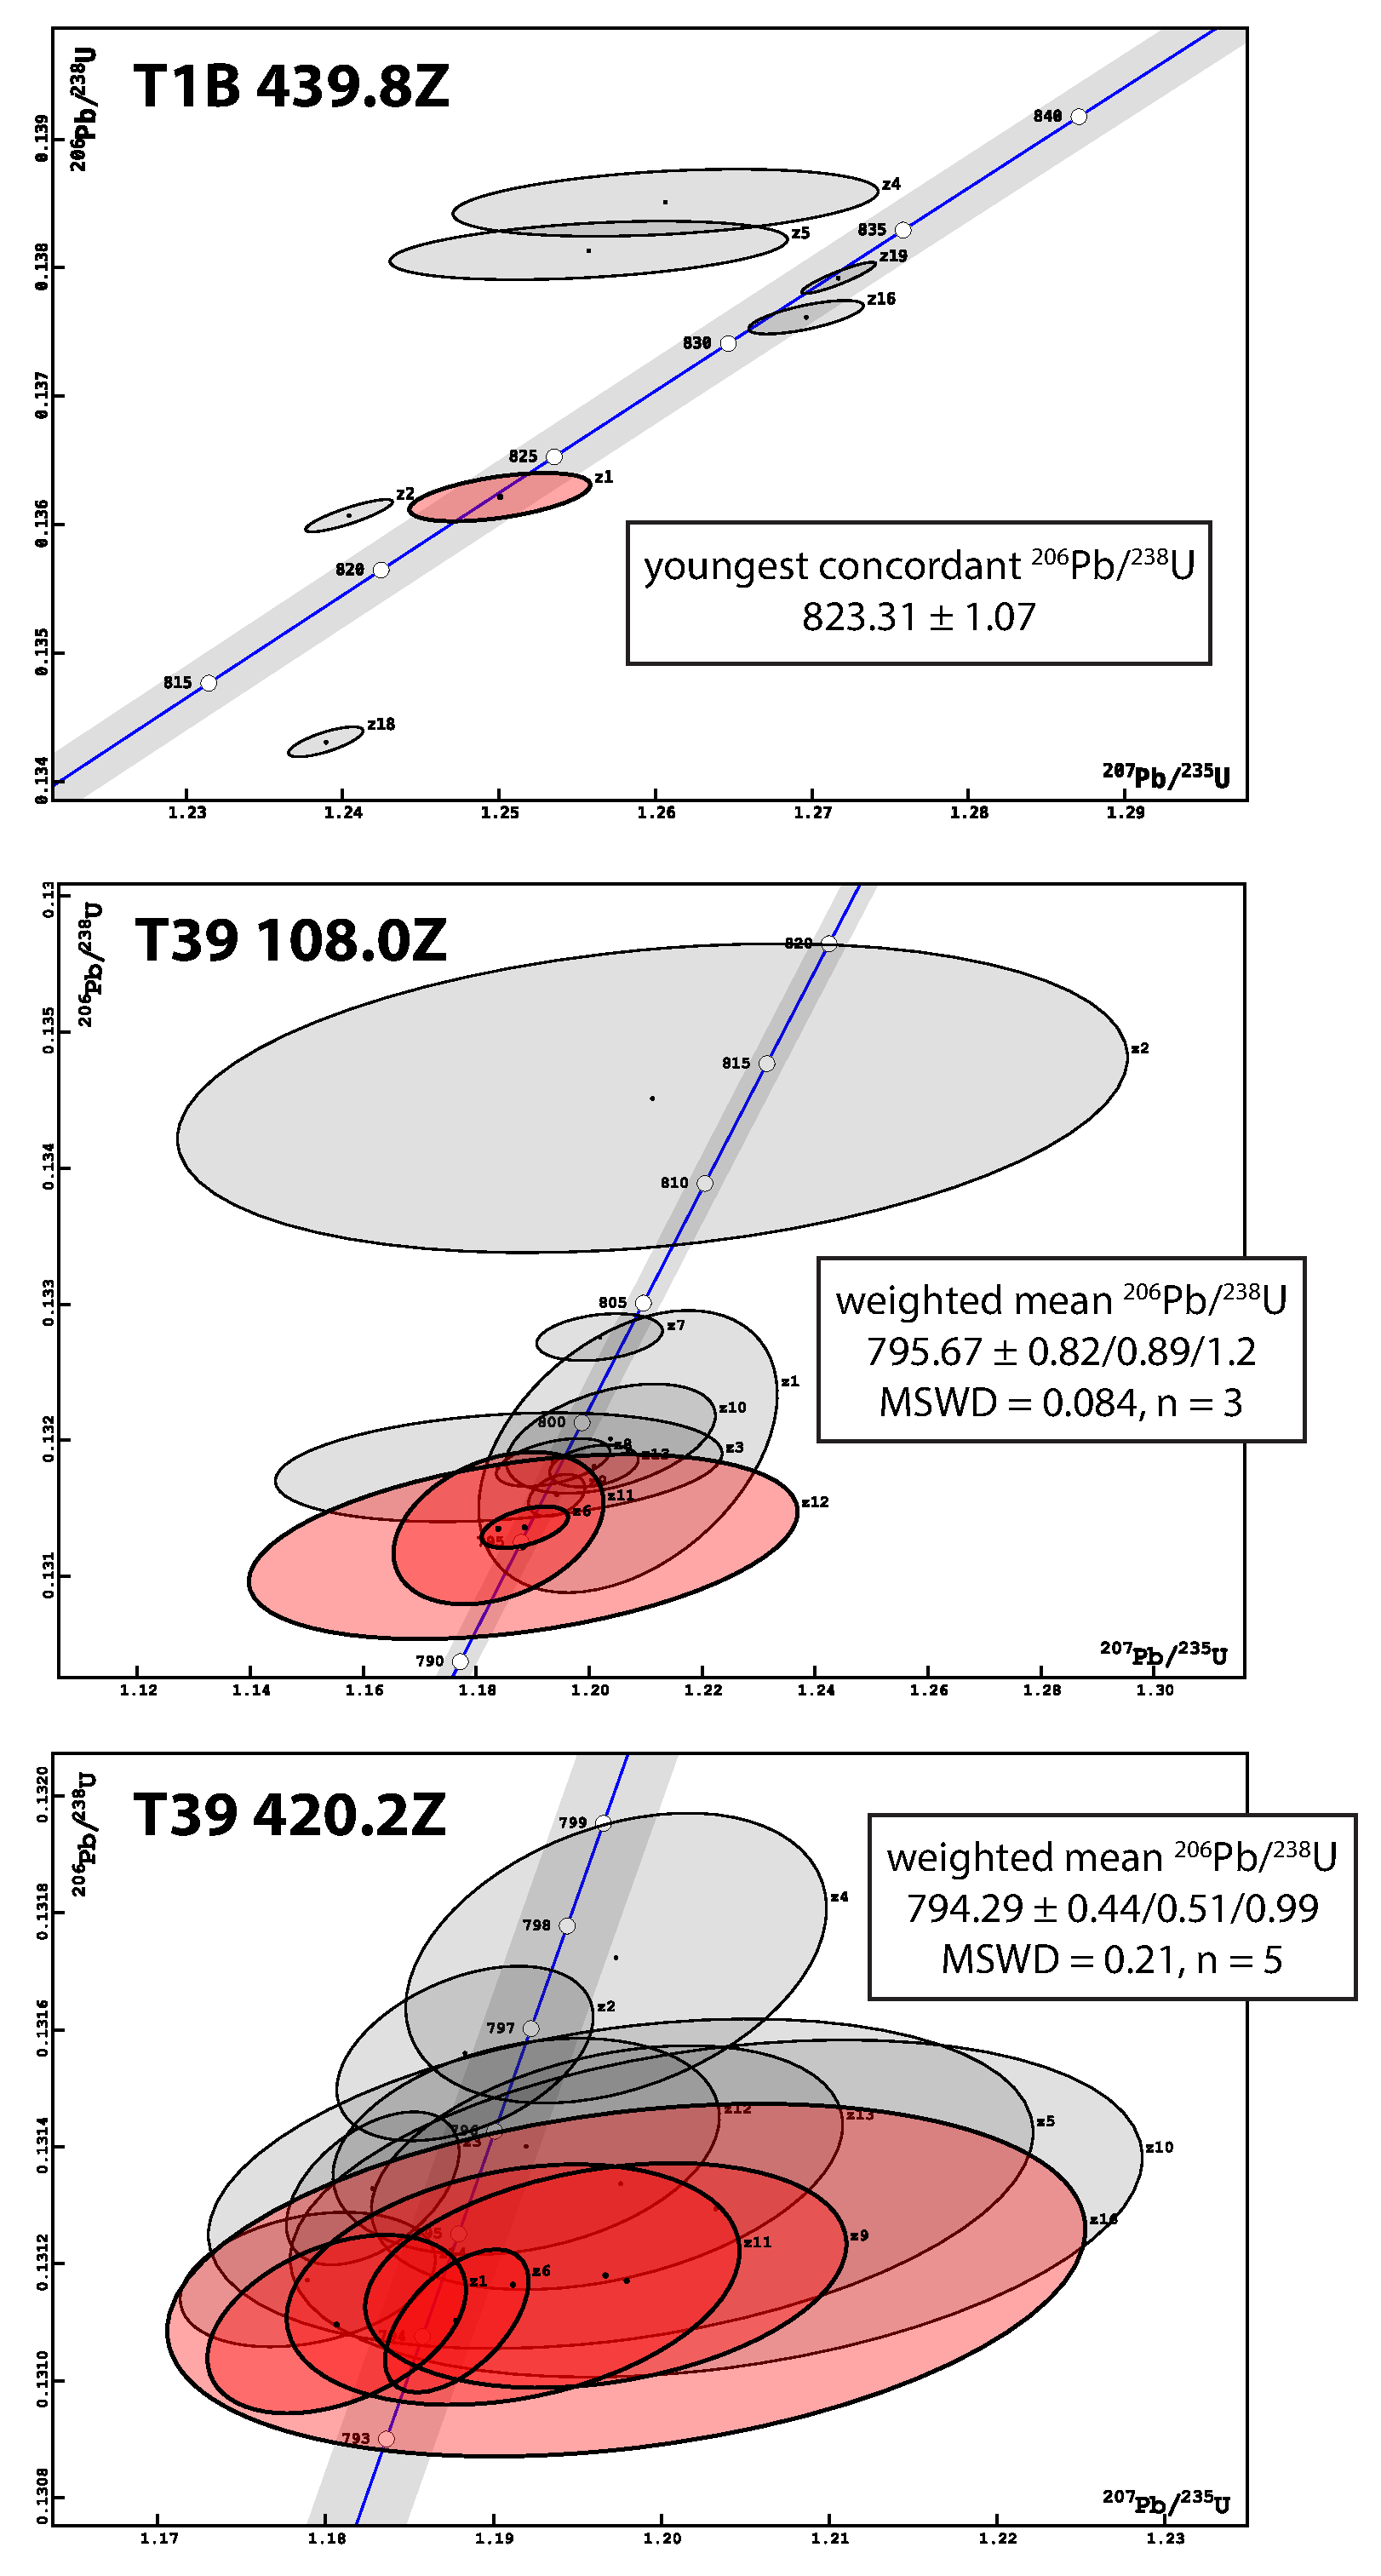
\includegraphics[width=0.5\textwidth]{Figures/Concordia.pdf}
	\caption{Concordia diagrams for dates reported in this study. 2$\sigma$ uncertainties are reported in the format $\pm$X/Y/Z, where X is the internal (analytical) uncertainty in the absence of all external or systematic errors, Y is the uncertainty incorporating the U-Pb tracer calibration error, and Z is the uncertainty including X and Y, as well as the uranium decay constant uncertainty; MSWD = mean square of weighted deviates; n = number of zircon analyses included in the calculated date.}
	\label{fig:Concordia}
\end{center}
\end{figure}

\begin{sidewaystable*}
\scriptsize
\vspace*{1 cm}
\caption{U-Pb data for analyzed zircon from T1B-439.8Z.}
\vspace{1 cm}
\setlength\tabcolsep{3.5pt}
\begin{tabular}{cccccccccccccccccccc}
& \multicolumn{8}{l}{Dates (Ma)} & \multicolumn{4}{l}{Composition} & \multicolumn{7}{l}{Isotopic Ratios} \\
\cline{2-20}\\
& $^a$ & & $^b$ & & $^{a,b}$ & & & $^c$ & $^d$ & $^e$ & $^f$ & $^{g}$ & $^h$ & $^{a,i}$ & & $^{b,i}$ & & $^{a,b,i}$ & \\	
& \underline{$^{206}$Pb} & $\pm$ & \underline{$^{207}$Pb} & $\pm$ & \underline{$^{207}$Pb} & $\pm$ & corr. & & \underline{Th} & Pb\** & Pb$_c$ & \underline{Pb\**} & \underline{$^{206}$Pb} & \underline{$^{206}$Pb} & $\pm$ & \underline{$^{207}$Pb} & $\pm$ & \underline{$^{207}$Pb} & $\pm$ \\		
fraction & $^{238}$U & (2$\sigma$) & $^{235}$U & (2$\sigma$) & $^{206}$Pb & (2$\sigma$) & coef. & \% disc. & U & (pg) & (pg) & Pb$_c$ & $^{204}$Pb & $^{238}$Pb & (2$\sigma\%$) & $^{235}$U & (2$\sigma\%$) & $^{206}$Pb & (2$\sigma\%$) \\
\hline \\  \vspace{0.2 cm}
\rowcolor{Yellow}
z1 & 823.31 & 1.07 & 823.43 & 2.61 & 823.76 & 8.55 & 0.51 & 0.10 & 0.34 & 23.13 & 0.61 & 37.96 & 2348.88 & 0.14 & 0.14 & 1.25 & 0.46 & 0.07 & 0.41 \\ \vspace{0.2 cm}
z2 & 822.49 & 0.71 & 819.07 & 1.26 & 809.80 & 3.20 & 0.85 & -1.53 & 0.35 & 68.32 & 0.62 & 110.86 & 6810.02 & 0.14 & 0.09 & 1.24 & 0.22 & 0.07 & 0.15 \\ \vspace{0.2 cm}
z4 & 836.29 & 1.48 & 828.20 & 6.10 & 806.54 & 21.58 & 0.33 & -3.65 & 0.53 & 13.16 & 0.86 & 15.23 & 908.36 & 0.14 & 0.19 & 1.26 & 1.08 & 0.07 & 1.03 \\ \vspace{0.2 cm}
z5 & 834.19 & 1.29 & 825.99 & 5.72 & 803.99 & 20.17 & 0.37 & -3.72 & 0.67 & 13.33 & 0.80 & 16.67 & 958.46 & 0.14 & 0.16 & 1.26 & 1.01 & 0.07 & 0.96 \\ \vspace{0.2 cm}
z16 & 831.24 & 0.74 & 832.22 & 1.64 & 834.86 & 4.89 & 0.69 & 0.47 & 0.65 & 13.75 & 0.22 & 61.23 & 3610.31 & 0.14 & 0.10 & 1.27 & 0.29 & 0.07 & 0.23 \\ \vspace{0.2 cm}
z17 & 855.05 & 0.73 & 855.83 & 1.17 & 857.86 & 2.59 & 0.92 & 0.36 & 0.73 & 32.33 & 0.18 & 181.54 & 10466.28 & 0.14 & 0.09 & 1.32 & 0.20 & 0.07 & 0.12 \\ \vspace{0.2 cm}
z18 & 812.48 & 0.67 & 818.40 & 1.08 & 834.51 & 2.95 & 0.73 & 2.67 & 0.75 & 42.34 & 0.32 & 130.41 & 7480.36 & 0.13 & 0.09 & 1.24 & 0.19 & 0.07 & 0.14 \\ \vspace{0.2 cm}
z19 & 832.98 & 0.69 & 833.16 & 1.06 & 833.64 & 2.36 & 0.90 & 0.12 & 0.57 & 47.38 & 0.18 & 266.55 & 15958.64 & 0.14 & 0.09 & 1.27 & 0.19 & 0.07 & 0.11 \\ \vspace{0.2 cm}
\end{tabular}

\flushleft \emph{Notes:} \\
Colored rows indicate fractions included in the calculation of the reported sample age. \\
Isotopic dates calculated using $\lambda$238 = 1.55125$\times$10$^{-10}$ and $\lambda$235 = 9.8485$\times$10$^{-10}$ \citep{Jaffey1971a}. \\
 $^{a}$  Corrected for initial Th/U disequilibrium using radiogenic $^{208}$Pb and Th/U[magma] = 3.50000. \\
 $^{b}$ Corrected for initial Pa/U disequilibrium using initial fraction activity ratio [$^{231}$Pa]/[$^{235}$U] = 1.10000. \\
 $^{c}$ \% discordance = 100 - (100 $\times$ ($^{206}$Pb/$^{238}$U date) / ($^{207}$Pb/$^{206}$Pb date)) \\
 $^{d}$ Th contents calculated from radiogenic $^{208}$Pb and $^{230}$Th-corrected $^{206}$Pb/$^{238}$U date of the sample, assuming concordance between U-Pb Th-Pb systems. \\
 $^{e}$ Total mass of radiogenic Pb. \\
 $^{f}$ Total mass of common Pb. \\
 $^{g}$ Ratio of radiogenic Pb (including $^{208}$Pb) to common Pb. \\
 $^{h}$ Measured ratio corrected for fractionation and spike contribution only. \\
 $^{i}$ Measured ratios corrected for fractionation, tracer and blank.
\end{sidewaystable*}

\begin{sidewaystable*}
\scriptsize
\vspace*{1 cm}
\caption{U-Pb data for analyzed zircon from T39-108.0Z.}
\vspace{1 cm}
\setlength\tabcolsep{3.5pt}
\begin{tabular}{cccccccccccccccccccc}
& \multicolumn{8}{l}{Dates (Ma)} & \multicolumn{4}{l}{Composition} & \multicolumn{7}{l}{Isotopic Ratios} \\
\cline{2-20}\\
& $^a$ & & $^b$ & & $^{a,b}$ & & & $^c$ & $^d$ & $^e$ & $^f$ & $^{g}$ & $^h$ & $^{a,i}$ & & $^{b,i}$ & & $^{a,b,i}$ & \\	
& \underline{$^{206}$Pb} & $\pm$ & \underline{$^{207}$Pb} & $\pm$ & \underline{$^{207}$Pb} & $\pm$ & corr. & & \underline{Th} & Pb\** & Pb$_c$ & \underline{Pb\**} & \underline{$^{206}$Pb} & \underline{$^{206}$Pb} & $\pm$ & \underline{$^{207}$Pb} & $\pm$ & \underline{$^{207}$Pb} & $\pm$ \\		
fraction & $^{238}$U & (2$\sigma$) & $^{235}$U & (2$\sigma$) & $^{206}$Pb & (2$\sigma$) & coef. & \% disc. & U & (pg) & (pg) & Pb$_c$ & $^{204}$Pb & $^{238}$Pb & (2$\sigma\%$) & $^{235}$U & (2$\sigma\%$) & $^{206}$Pb & (2$\sigma\%$) \\
\hline \\  \vspace{0.2 cm}
z1 & 798.88 & 5.90 & 803.74 & 12.16 & 817.26 & 41.88 & 0.41 & 2.29 & 0.57 & 1.59 & 0.25 & 6.29 & 395.48 & 0.13 & 0.79 & 1.21 & 2.19 & 0.07 & 2.00 \\ \vspace{0.2 cm}
z2 & 813.64 & 6.45 & 805.73 & 38.62 & 783.94 & 142.22 & 0.26 & -3.75 & 0.56 & 0.54 & 0.30 & 1.78 & 125.78 & 0.13 & 0.84 & 1.21 & 6.94 & 0.07 & 6.77 \\ \vspace{0.2 cm}
z3 & 798.22 & 2.28 & 793.16 & 18.38 & 778.96 & 68.88 & 0.25 & -2.43 & 0.51 & 4.01 & 1.13 & 3.54 & 233.74 & 0.13 & 0.30 & 1.18 & 3.34 & 0.07 & 3.28 \\ \vspace{0.2 cm}
\rowcolor{Yellow}
z6 & 795.71 & 0.87 & 795.30 & 3.56 & 794.14 & 12.54 & 0.49 & -0.16 & 0.47 & 5.66 & 0.27 & 20.81 & 1297.81 & 0.13 & 0.12 & 1.19 & 0.65 & 0.07 & 0.60 \\ \vspace{0.2 cm}
z7 & 803.66 & 0.98 & 801.43 & 5.14 & 795.22 & 18.90 & 0.27 & -1.02 & 0.43 & 4.03 & 0.31 & 12.82 & 813.30 & 0.13 & 0.13 & 1.20 & 0.93 & 0.07 & 0.90 \\ \vspace{0.2 cm}
z8 & 798.42 & 1.01 & 797.63 & 4.66 & 795.41 & 16.56 & 0.46 & -0.34 & 0.58 & 5.09 & 0.31 & 16.30 & 993.36 & 0.13 & 0.13 & 1.19 & 0.84 & 0.07 & 0.79 \\ \vspace{0.2 cm}
z9 & 797.04 & 0.88 & 797.93 & 2.31 & 800.40 & 8.21 & 0.36 & 0.46 & 0.73 & 12.47 & 0.33 & 38.31 & 2223.30 & 0.13 & 0.12 & 1.19 & 0.42 & 0.07 & 0.39 \\ \vspace{0.2 cm}
z10 & 799.42 & 2.28 & 802.34 & 8.53 & 810.47 & 30.06 & 0.42 & 1.40 & 0.50 & 2.01 & 0.20 & 10.01 & 628.68 & 0.13 & 0.30 & 1.20 & 1.54 & 0.07 & 1.44 \\ \vspace{0.2 cm}
\rowcolor{Yellow}
z11 & 795.67 & 3.19 & 793.15 & 8.65 & 786.05 & 31.21 & 0.33 & -1.18 & 0.44 & 2.11 & 0.27 & 7.93 & 509.16 & 0.13 & 0.43 & 1.18 & 1.57 & 0.07 & 1.49 \\ \vspace{0.2 cm}
\rowcolor{Yellow}
z12 & 794.90 & 3.87 & 795.18 & 22.55 & 795.97 & 82.26 & 0.38 & 0.18 & 0.42 & 1.37 & 0.39 & 3.54 & 238.72 & 0.13 & 0.52 & 1.19 & 4.09 & 0.07 & 3.92 \\ \vspace{0.2 cm}
z13 & 798.28 & 0.88 & 800.97 & 3.63 & 808.48 & 13.15 & 0.31 & 1.30 & 0.43 & 5.40 & 0.28 & 19.34 & 1218.11 & 0.13 & 0.12 & 1.20 & 0.65 & 0.07 & 0.63 \\ \vspace{0.2 cm}
\end{tabular}

\flushleft \emph{Notes:} \\
Colored rows indicate fractions included in the calculation of the reported sample age. \\
Isotopic dates calculated using $\lambda$238 = 1.55125$\times$10$^{-10}$ and $\lambda$235 = 9.8485$\times$10$^{-10}$ \citep{Jaffey1971a}. \\
 $^{a}$  Corrected for initial Th/U disequilibrium using radiogenic $^{208}$Pb and Th/U[magma] = 3.50000. \\
 $^{b}$ Corrected for initial Pa/U disequilibrium using initial fraction activity ratio [$^{231}$Pa]/[$^{235}$U] = 1.10000. \\
 $^{c}$ \% discordance = 100 - (100 $\times$ ($^{206}$Pb/$^{238}$U date) / ($^{207}$Pb/$^{206}$Pb date)) \\
 $^{d}$ Th contents calculated from radiogenic $^{208}$Pb and $^{230}$Th-corrected $^{206}$Pb/$^{238}$U date of the sample, assuming concordance between U-Pb Th-Pb systems. \\
 $^{e}$ Total mass of radiogenic Pb. \\
 $^{f}$ Total mass of common Pb. \\
 $^{g}$ Ratio of radiogenic Pb (including $^{208}$Pb) to common Pb. \\
 $^{h}$ Measured ratio corrected for fractionation and spike contribution only. \\
 $^{i}$ Measured ratios corrected for fractionation, tracer and blank.
\end{sidewaystable*}

\begin{sidewaystable*}
\scriptsize
\vspace*{1 cm}
\caption{U-Pb data for analyzed zircon from T39-420.2Z.}
\vspace{1 cm}
\setlength\tabcolsep{3.5pt}
\begin{tabular}{cccccccccccccccccccc}
& \multicolumn{8}{l}{Dates (Ma)} & \multicolumn{4}{l}{Composition} & \multicolumn{7}{l}{Isotopic Ratios} \\
\cline{2-20}\\
& $^a$ & & $^b$ & & $^{a,b}$ & & & $^c$ & $^d$ & $^e$ & $^f$ & $^{g}$ & $^h$ & $^{a,i}$ & & $^{b,i}$ & & $^{a,b,i}$ & \\	
& \underline{$^{206}$Pb} & $\pm$ & \underline{$^{207}$Pb} & $\pm$ & \underline{$^{207}$Pb} & $\pm$ & corr. & & \underline{Th} & Pb\** & Pb$_c$ & \underline{Pb\**} & \underline{$^{206}$Pb} & \underline{$^{206}$Pb} & $\pm$ & \underline{$^{207}$Pb} & $\pm$ & \underline{$^{207}$Pb} & $\pm$ \\		
fraction & $^{238}$U & (2$\sigma$) & $^{235}$U & (2$\sigma$) & $^{206}$Pb & (2$\sigma$) & coef. & \% disc. & U & (pg) & (pg) & Pb$_c$ & $^{204}$Pb & $^{238}$Pb & (2$\sigma\%$) & $^{235}$U & (2$\sigma\%$) & $^{206}$Pb & (2$\sigma\%$) \\
\hline \\  \vspace{0.2 cm}
\rowcolor{Yellow}
z1 & 794.12 & 0.87 & 791.62 & 3.59 & 784.58 & 12.98 & 0.38 & -1.18 & 0.69 & 11.98 & 0.49 & 24.28 & 1391.39 & 0.13 & 0.12 & 1.18 & 0.65 & 0.07 & 0.62 \\ \vspace{0.2 cm}
z2 & 796.76 & 0.85 & 795.17 & 3.55 & 790.74 & 12.69 & 0.42 & -0.73 & 0.87 & 15.22 & 0.59 & 25.79 & 1415.45 & 0.13 & 0.11 & 1.19 & 0.64 & 0.07 & 0.60 \\ \vspace{0.2 cm}
z3 & 795.44 & 0.75 & 792.62 & 2.40 & 784.69 & 8.35 & 0.48 & -1.33 & 0.76 & 23.62 & 0.59 & 40.01 & 2239.52 & 0.13 & 0.10 & 1.18 & 0.44 & 0.07 & 0.40 \\ \vspace{0.2 cm}
z4 & 797.69 & 1.41 & 799.35 & 5.80 & 803.97 & 20.92 & 0.34 & 0.82 & 0.73 & 13.69 & 0.91 & 15.02 & 857.80 & 0.13 & 0.19 & 1.20 & 1.05 & 0.07 & 1.00 \\ \vspace{0.2 cm}
z5 & 795.49 & 1.61 & 799.47 & 11.36 & 810.60 & 41.75 & 0.31 & 1.90 & 0.64 & 12.24 & 1.71 & 7.15 & 427.13 & 0.13 & 0.21 & 1.20 & 2.05 & 0.07 & 2.00 \\ \vspace{0.2 cm}
\rowcolor{Yellow}
z6 & 794.15 & 0.70 & 794.95 & 1.99 & 797.18 & 6.68 & 0.55 & 0.42 & 0.77 & 43.52 & 0.87 & 50.28 & 2801.05 & 0.13 & 0.09 & 1.19 & 0.36 & 0.07 & 0.32 \\ \vspace{0.2 cm}
\rowcolor{Yellow}
z9 & 794.59 & 1.09 & 799.06 & 6.63 & 811.54 & 24.38 & 0.28 & 2.12 & 1.20 & 8.79 & 0.62 & 14.19 & 731.99 & 0.13 & 0.15 & 1.20 & 1.20 & 0.07 & 1.17 \\ \vspace{0.2 cm}
z10 & 795.25 & 1.64 & 802.10 & 11.70 & 821.19 & 42.92 & 0.30 & 3.19 & 1.06 & 10.65 & 1.38 & 7.70 & 416.84 & 0.13 & 0.22 & 1.20 & 2.11 & 0.07 & 2.06 \\ \vspace{0.2 cm}
\rowcolor{Yellow}
z11 & 794.51 & 1.17 & 796.51 & 6.26 & 802.10 & 23.04 & 0.28 & 0.98 & 0.69 & 5.42 & 0.40 & 13.43 & 776.60 & 0.13 & 0.16 & 1.19 & 1.13 & 0.07 & 1.10 \\ \vspace{0.2 cm}
z12 & 795.85 & 1.05 & 796.87 & 5.34 & 799.70 & 19.65 & 0.27 & 0.51 & 1.16 & 10.71 & 0.61 & 17.46 & 903.55 & 0.13 & 0.14 & 1.19 & 0.97 & 0.07 & 0.94 \\ \vspace{0.2 cm}
z13 & 795.65 & 1.19 & 799.10 & 6.49 & 808.72 & 23.61 & 0.35 & 1.65 & 0.66 & 5.25 & 0.40 & 13.04 & 760.42 & 0.13 & 0.16 & 1.20 & 1.17 & 0.07 & 1.13 \\ \vspace{0.2 cm}
z14 & 794.55 & 0.66 & 790.82 & 3.54 & 780.29 & 13.14 & 0.29 & -1.80 & 1.30 & 10.90 & 0.40 & 27.31 & 1363.19 & 0.13 & 0.09 & 1.18 & 0.64 & 0.07 & 0.62 \\ \vspace{0.2 cm}
\rowcolor{Yellow}
z16 & 794.55 & 1.72 & 799.63 & 12.64 & 813.80 & 46.60 & 0.29 & 2.40 & 0.66 & 7.30 & 1.14 & 6.40 & 382.41 & 0.13 & 0.23 & 1.20 & 2.28 & 0.07 & 2.23 \\ \vspace{0.2 cm}
\end{tabular}

\flushleft \emph{Notes:} \\
Colored rows indicate fractions included in the calculation of the reported sample age. \\
Isotopic dates calculated using $\lambda$238 = 1.55125$\times$10$^{-10}$ and $\lambda$235 = 9.8485$\times$10$^{-10}$ \citep{Jaffey1971a}. \\
 $^{a}$  Corrected for initial Th/U disequilibrium using radiogenic $^{208}$Pb and Th/U[magma] = 3.50000. \\
 $^{b}$ Corrected for initial Pa/U disequilibrium using initial fraction activity ratio [$^{231}$Pa]/[$^{235}$U] = 1.10000. \\
 $^{c}$ \% discordance = 100 - (100 $\times$ ($^{206}$Pb/$^{238}$U date) / ($^{207}$Pb/$^{206}$Pb date)) \\
 $^{d}$ Th contents calculated from radiogenic $^{208}$Pb and $^{230}$Th-corrected $^{206}$Pb/$^{238}$U date of the sample, assuming concordance between U-Pb Th-Pb systems. \\
 $^{e}$ Total mass of radiogenic Pb. \\
 $^{f}$ Total mass of common Pb. \\
 $^{g}$ Ratio of radiogenic Pb (including $^{208}$Pb) to common Pb. \\
 $^{h}$ Measured ratio corrected for fractionation and spike contribution only. \\
 $^{i}$ Measured ratios corrected for fractionation, tracer and blank.
\end{sidewaystable*}

\begin{figure}[h!]
\begin{center}
	\includegraphics[width=\textwidth]{Figures/Geochronology_Photos.jpg}
	\caption{\textbf{(A)} Photograph of the lava flow T1b-439.8Z. \textbf{(B)} Photograph of the ignimbrite T39-108.0Z, with feldspar phenocrysts and fiammed lithic clasts. \textbf{(C)} Photograph of the 30~cm rhyolitic tuff T39-420.2Z, with normally graded lapilli at the base. Hammer points up section in all panels.}
	\label{fig:Geochronology_Photos}
\end{center}
\end{figure}

\clearpage

\section*{Diagenetic Considerations}

\subsection*{Isotope Conglomerate Test}

\begin{figure}[h!]
\begin{center}
	\includegraphics[width=\textwidth]{Figures/Clast_Analysis_Pval.pdf}
	\caption{\textbf{(A)} and \textbf{(B)} Histograms of \dC and \dO values of carbonate clasts within the diamictite of the Negash Formation of both the Negash Syncline and Samre Fold-Thrust Belt, compared to all \textit{in situ} Tambien Group carbonate samples. Both filtered and unfiltered (all) versions of the \textit{in situ} carbonate data are shown (see main text for a discussion of the filtering method). \textbf{(C)} and \textbf{(D)} Cross plots of \dC vs \dO for the clasts and \textit{in situ} carbonate samples. \textbf{(E)} Filtered and unfiltered versions of the \textit{in situ} carbonate \dC data against cumulative stratigraphic height. \textbf{(F)} Degree of correlation (as quantified by the Kolgomorov-Smirnov statistic) between the \textit{in situ} carbonate \dC data with the carbonate clasts within the diamictite as samples below a given cumulative stratigraphic height (x-axis) are removed (i.e. the x-axis represents the depth of erosion). Low values suggest that the two datasets are drawn from the same distribution. See accompanying text for further details. \textbf{(G)} Kolgomorov-Smirnov statistic p-value. High values suggest that the two datasets are drawn from the same distribution.}
	\label{fig:Clast_Analysis_Pval}
\end{center}
\end{figure}

We compare \dC and \dO values of the carbonate clasts from within diamictite of the Negash Formation of the Negash Syncline and Samre Fold-Thrust Belt. In general, the distribution of clast \dC values is similar to that of the \textit{in situ} Tambien Group carbonates (Fig. \ref{fig:Clast_Analysis_Pval}A). However, the filtering technique proposes that the stratigraphic distance of a sample to the closest siliciclastic unit is a reasonable predictor for \dC alteration in \textit{in situ} Tambien Group carbonates. If such a scenario applied equally to the diamictite clasts, we might expect the \dC of the clasts to be pulled to more negative values relative to the \textit{in situ} carbonates since most of the samples in the \textit{in situ} stratigraphy were extracted from carbonate horizons thicker than the diamictite clasts, but such a distribution is not observed.

There are several potential explanations for this apparent inconsistency. First, as discussed in the main text, samples that fall below the threshold \dsil may or may not have had their carbon isotopic composition altered. And so, even though the majority of sampled diamictite clasts have a radius \textless0.2~m, the \dC of a significant proportion of these samples need not have been affected by secondary alteration. Second, it is possible that carbon is better buffered in the diamictite relative to the rest of the Tambien Group. Unless 100\% of the diamictite's matrix was produced via scouring and redeposition of pre-Snowball Earth siliciclastics with associated organic matter, the matrix likely contains less low \dC organic carbon relative to the siliciclastic units of the underlying Tambien Group, given that organic productivity was suppressed during the Snowball Earth \citep{Hoffman2017a}. The presence of extra-basinal clasts within the diamictite (see main text) suggests that at least some of the protolith was sourced from distal bedrock, and thus the organic component of the diamictite's matrix was likely diluted relative to undisturbed Tambien Group siliciclastics. Third, given that glacial erosion generates a bimodal sediment size distribution (fine grains from scouring and larger clasts from plucking) from the same rock, the sampled carbonate clasts in the diamictite are likely accompanied by fine carbonate sand from the same rock. This relatively carbonate-rich diamictite matrix would help to buffer the carbon isotopic composition of diamictite clasts against changes in \dC in a way that siliciclastic units within the \textit{in situ} Tambien Group stratigraphy would not be able to. Finally, it is possible that our sampling of clasts from the diamictite is not representative of the bulk population. The total number of diamictite clasts sampled (n = 78) is substantially smaller than the total number of samples from \textit{in situ} Tambien Group carbonates (n = 3139). Furthermore, diamictite clasts were only sampled from three discrete stratigraphic horizons, which may have been more carbonate buffered relative to the rest of the diamictite.

\dO values of the diamictite clasts are distinctly different from the spread in values observed in the \textit{in situ} stratigraphy, and cluster at $\sim$-12\permil (Fig. \ref{fig:Clast_Analysis_Pval}B). This difference suggests that, unlike the carbon isotopic composition, the oxygen isotope composition of the carbonate clasts was significantly more overprinted following deposition of the diamictite than that of the \textit{in situ} carbonates. This difference in post-depositional alteration likely arises from the fact that the carbonate clasts in the diamictite are embedded within a predominantly siliciclastic matrix and are therefore less carbonate buffered against altering fluids, whereas most of the samples in the \textit{in situ} stratigraphy were extracted from carbonate horizons thicker than the diamictite clasts and are therefore more likely to be carbonate buffered. Since carbon is more rock-buffered against altering fluids than oxygen, the \dC of the clasts are more likely to preserve primary values.

Glacial erosion during the Sturtian Glaciation likely preferentially eroded the upper Tambien Group in most places instead of eroding all the way to the base of the Tambien Group. To assess how deep the bulk of glaciers eroded into Tambien Group stratigraphy, we divided the Tambien Group chemostratigraphic composite data collected from the \textit{in situ} stratigraphy (Fig. \ref{fig:Clast_Analysis_Pval}E) into several equal length (50~m) stratigraphic windows, and randomly selected the same number of samples from each of these windows. This Monte Carlo approach is necessary to avoid bias toward relatively heavily sampled intervals of the stratigraphy. We then quantified the similarity in distributions between the \dC of the Monte Carlo sampled \textit{in situ} stratigraphy with that of the diamictite clasts using the two sample Kolmogorov-Smirnov (KS) statistic, which tests whether two sets of samples are consistent with being drawn from the same distribution. Low KS statistics and high p-values suggest that the two samples are drawn from the same distribution. We then simulate shallower erosion by iteratively excluding the lowest of these stratigraphic windows and recalculating the KS statistic, moving up the stratigraphy (Fig. \ref{fig:Clast_Analysis_Pval}F and G). In general, we find that the two distributions are closest when the `erosion height' is close to the bottom of the Tambien Group ($\sim$0~m in Fig. \ref{fig:Clast_Analysis_Pval}F and G) and near the middle of the Tambien Group ($\sim$2900~m). We also observe a distinct trough/peak near the top of the Tambien Group ($\sim$4200~m), although the KS statistic/p-value is not as low/high as at the bottom or near the middle of the Tambien Group. Furthermore, the filtered version of the \textit{in situ} carbonate \dC data (see main text) matches the clast data more poorly than all of the \textit{in situ} carbonate \dC data, likely as a result of similar post-depositional alteration mechanisms operating throughout the entirety of the Tambien Group. Ultimately, this analysis illustrates the fact that a relatively large proportion of the diamictite clasts have relatively low \dC (\textless0\permil), and thus the clast \dC distribution matches the \textit{in situ} carbonate \dC distribution when the `erosion height' is such that it includes a high proportion of samples within the Bitter Springs Stage, the Islay Anomaly, and/or carbonate samples that have likely experienced secondary alteration pulling them to lower \dC values. Observations of the facies of clasts within the diamictite suggest that they were sourced predominantly from the Matheos and/or Mariam Bohkahko formations (see main text), and thus an `erosion height' of $\sim$2900~m or $\sim$4200~m would be consistent with these facies. The KS statistic/p-value at these `erosion heights' is low/high enough such that we cannot reject the null hypothesis that the diamictite clasts and the \textit{in situ} carbonate samples from above these heights come from the same distribution. However, we note that erosion into the Mariam Bohkahko/Matheos formations is not observed locally where the diamictite is deposited. This observation requires that the clasts derive from carbonates time-equivalent to these formations deposited elsewhere in the basin, or from carbonates deposited in another basin within an Arabian-Nubian terrane.

\clearpage

\subsection*{Filtering Samples Adjacent to Siliciclastic Units}

\begin{figure}[h!]
\begin{center}
	\includegraphics[width=0.7\textwidth]{Figures/MTS_MTX_Comparison.pdf}
	\caption{Cross plots of carbonate matrix vs. adjacent molar tooth structure calcite \SrSr and \dC from Tambien Group samples that meet the filtering thresholds for alteration (see main text). Dashed black lines are the 1:1 lines - samples that fall on these lines have identical isotopic composition between the matrix and molar tooth structure carbonate. The isotopic composition of the matrix is similar to that of adjacent molar tooth structures, and no systematic offsets can be identified.}
	\label{fig:MTS_MTX_comparison}
\end{center}
\end{figure}

\begin{figure}[h!]
\begin{center}
	\includegraphics[width=0.5\textwidth]{Figures/Siliciclastic_Filtering_Components.pdf}
	\caption{Eigenvalues and cumulative variance explained for the 7 principal components in the principal components analysis (also known as a scree plot). Notably, the magnitude of the eigenvalues (and the percent variance explained) drops off sharply after the second principal component, indicating that the first two principal components capture the most significant sources of variance in our dataset.}
	\label{fig:Siliciclastic_Filtering_Components}
\end{center}
\end{figure}

\begin{figure}[h!]
\begin{center}
	\includegraphics[width=\textwidth]{Figures/Siliciclastic_Filtering_Comparison.pdf}
	\caption{Resulting composite chemostratigraphy of the Tambien Group as samples below a given \dsil (shown on the right) are filtered out. Note that data that resolve the Islay Anomaly as well as the descent into and recovery out of the Bitter Springs Stage are mostly removed under the \dsil = 0.2~m threshold, and completely removed by \dsil = 0.5~m.}
	\label{fig:Siliciclastic_Filtering_Comparison}
\end{center}
\end{figure}

\begin{figure}[h!]
\begin{center}
	\includegraphics[width=\textwidth]{Figures/Siliciclastic_Filtering_Islay.pdf}
	\caption{Comparison of individual samples above the Islay Anomaly vs. samples within/adjacent to the Islay Anomaly. The normalized histograms under each scatter plot compare the distribution of samples with \dC$\leq$0\permil only. The `stat.' and `p-val.' refer to the Kolmogorov-Smirnov statistic and p-value respectively, with the value within the parentheses showing the critical Kolmogorov-Smirnov statistic for rejecting the null hypothesis (see text below).}
	\label{fig:Siliciclastic_Filtering_Islay}
\end{center}
\end{figure}

\clearpage

As per conventions in statistics, the following discussion will use the term `unit' to refer to an individual carbonate rock, and the term `sample' to refer to a collection of `units' from a population. Figure \ref{fig:Siliciclastic_Filtering_Islay} compares geochemical data of units above the Islay Anomaly to units within/adjacent to the Islay Anomaly. Units within the Islay Anomaly that record \dC$\leq$0\permil appear to exhibit lower Fe, Al, and Mn/Sr than units that record \dC$\leq$0\permil above the Islay Anomaly. This difference in distributions suggests that low \dC Islay Anomaly units have been less altered by the unbuffered fluids (see main text) than low \dC post-Islay Anomaly units, and thus provides support for the primary nature of the anomaly. To quantify this qualitative interpretation of the data, we compare the distributions of units with low \dC above the Islay Anomaly to units with low \dC within the Islay Anomaly by computing the two-sample Kolmogorov-Smirnov (KS) statistic. We also compute the critical KS statistic for rejecting the null hypothesis, which is given by $1.36\sqrt{\frac{N_{1}+N_{2}}{N_{1}N_{2}}}$, where $N_{1}$ and $N_{2}$ are the number of items in the two samples. If the computed KS statistic is above the critical KS statistic, or the p-value is below 0.05, we can reject the null hypothesis at the 95\% confidence level that the two samples come from the same distribution. We find that the KS test yields ambiguous results for the Fe, Al, and Mn/Sr (Fig. \ref{fig:Siliciclastic_Filtering_Islay}). For all three variables, the KS statistic is below the critical value, and the p-value is above 0.05. These results indicate that we cannot declare at the 95\% confidence level that the two samples come from different distributions - instead, the test indicates that the samples may or may not come from the same distribution. However, the primary reason for this ambiguity is the small number of units used in the test. There are only 20 units with \dC$\leq$0\permil and element concentration data above the Islay Anomaly, and only 9 units with \dC$\leq$0\permil and element concentration within the Islay Anomaly, which results in a high critical KS statistic and thus a more `difficult' test to achieve an unambiguous result in. Therefore, more element concentration data is required in order for the KS test to quantitatively reject the hypothesis at the 95\% confidence level that units within the Islay Anomaly that record \dC$\leq$0\permil exhibit lower Fe, Al, and Mn/Sr than units that record \dC$\leq$0\permil above the Islay Anomaly.

\clearpage

\subsection*{Sr Isotopes}

\begin{figure}[h!]
\begin{center}
	\includegraphics[width=0.8\textwidth]{Figures/Filter_Comparison.pdf}
	\caption{Comparison of the application of the [Sr] and Mn/Sr filter and the filter based on distance to siliciclastics (\dsil) to the \SrSr data, for both \dsil = 0.2~m and \dsil = 0.5~m. Orange sectors denote classification agreement between the two filters, and grey sectors denote classification disagreement between the two filters. In the upper row, both the [Sr] and Mn/Sr thresholds are combined to filter samples. In the lower row, only the Mn/Sr threshold is used to filter samples.}
	\label{fig:Filter_Comparison}
\end{center}
\end{figure}

Figure \ref{fig:Filter_Comparison} compares the application of the [Sr] and Mn/Sr filter and the filter based on distance to siliciclastics (\dsil) to the \SrSr data. When both the [Sr] and Mn/Sr thresholds are combined to filter samples (as in the main text), the [Sr] and Mn/Sr filter and the \dsil filter only agree on classification for around half of the samples. This lack of agreement results from the fact that the principal components analysis used for the \dsil filter (see main text) includes Mn/Sr, and not [Sr], as a variable in the analysis, since [Sr] in carbonates can vary considerably based on factors other than secondary alteration (e.g. calcite vs. aragonite, \citealp{Husson2015b}). Therefore, by using the Mn/Sr threshold only to filter samples, agreement between the Mn/Sr filter and the \dsil filter improves. Still, considerable disagreement between the two filters remain, which highlights the limitations of the \dsil filter as discussed in the main text. Namely, that in addition to filtering out samples that have been altered, it is a rather blunt filter and may also filter out samples that retain relatively pristine geochemistry.

\section*{Pre-Sturtian \SrSr and the Drivers of Planetary Cooling}

\subsection*{LIP Analysis}

\begin{sidewaystable*}
\scriptsize
\vspace*{1 cm}
\caption{Large igneous provinces included in the analysis conducted in the main text.}
\vspace{1 cm}
    \resizebox{\linewidth}{!}{
	\begin{tabular}{l l c c c l l l}
    \textbf{Name} & \textbf{Craton} & \textbf{Emplacement} & \textbf{Emplacement} & \textbf{Polygon Centroid} & \textbf{Age Reference} & \textbf{Polygon Reference} & \textbf{Paleomagnetic Pole} \\
    & & \textbf{Age [Ma]} & \textbf{Area [Mkm$^{2}$]} & \textbf{Emplacement Latitude} & & & \textbf{Reference} \\
    \hline \\ \vspace{0.2 cm}
    Mackenzie & Laurentia & 1267 & 2.983 & 11.4 & \citet{LeCheminant1989a} & \citet{Ernst2017a} & \citet{Buchan2000a} \\ \vspace{0.2 cm}
    CSDG & Baltica & 1255 & 0.145 & -24 & \citet{Soderlund2006a} & \citet{Ernst2017a} & \citet{Pisarevsky2014b} \\ \vspace{0.2 cm}
    Sudbury & Laurentia & 1235 & 0.056 & 7.7 & \citet{Dudas1994a} & \citet{Shellnutt2012a} & \citet{Palmer1977a} \\ \vspace{0.2 cm}
    Marnda Moorn & SW. Australia & 1210 & 0.598 & 65.2 & \citet{Pisarevsky2014a} & \citet{Ernst2017a} & \citet{Pisarevsky2014a} \\ \vspace{0.2 cm}
    Abitibi & Laurentia & 1141 & 0.229 & 48.2 & \citet{Krogh1987a} & \citet{Ernst2017a} & \citet{Ernst1993a} \\ \vspace{0.2 cm}
    Umkondo & Kalahari & 1109 & 1.846 & 0.8 & \citet{Hanson2004a} & \citet{Ernst2017a} & \citet{Swanson-Hysell2015b} \\ \vspace{0.2 cm}
    Keweenawan & Laurentia & 1109 & 0.414 & 41.9 & \citet{Davis1997a} & \citet{Ernst2017a} & \citet{Swanson-Hysell2014b} \\ \vspace{0.2 cm}
    SW Laurentia & Laurentia & 1090 & 0.776 & 28.7 & \citet{Weil2003a} & \citet{Bright2014a} & \citet{Weil2003a} \\ \vspace{0.2 cm}
    Warakurna - 1 & SW. + N. Australia & 1070 & 0.757 & 38.6 & \citet{Wingate2002a} & \citet{Ernst2017a} & \citet{Wingate2002a} \\ \vspace{0.2 cm}
    Warakurna - 2 & SW. + N. Australia & 1070 & 0.444 & 41.9 & \citet{Wingate2002a} & \citet{Ernst2017a} & \citet{Wingate2002a} \\ \vspace{0.2 cm}
    Dashigou & N. China & 925 & 0.663 & 3.9 & \citet{Peng2011a} & \citet{Pirajno2013a} & - \\ \vspace{0.2 cm}
    Gangil-Mayumbia & Congo & 920 & 0.333 & -52.3 & \citet{Tack2001a} & \citet{Ernst2017a} & - \\ \vspace{0.2 cm}
    Willouran-Gairdner - 1 & S. Australia & 827 & 0.345 & 24.3 & \citet{Wingate1998a} & \citet{Ernst2017a} & - \\ \vspace{0.2 cm}
    Willouran-Gairdner - 2 & S. Australia & 827 & 0.171 & 29.3 & \citet{Wingate1998a} & \citet{Ernst2017a} & - \\ \vspace{0.2 cm}
    SWCUC - 1 & S. China & 821 & 0.914 & 68.6 & \citet{Wang2016b} & \citet{Ernst2017a} & \citet{Li2004a} \\ \vspace{0.2 cm}
    SWCUC - 2 & S. China & 821 & 0.411 & 65.6 & \citet{Wang2016b} & \citet{Ernst2017a} & \citet{Li2004a} \\ \vspace{0.2 cm}
    Gunbarrel - 1 & Laurentia & 780 & 0.21 & -7 & \citet{Harlan2003a} & \citet{Ernst2017a} & \citet{Park1989a} \\ \vspace{0.2 cm}
    Gunbarrel - 2 & Laurentia & 780 & 0.34 & 4.2 & \citet{Harlan2003a} & \citet{Ernst2017a} & \citet{Park1989a} \\ \vspace{0.2 cm}
    Mundine Well & N. Australia & 755 & 0.21 & 25.6 & \citet{Wingate2000a} & \citet{Ernst2017a} & \citet{Wingate2000a} \\ \vspace{0.2 cm}
    Irkutsk & Siberia & 724 & 0.154 & 13.6 & \citet{Ernst2016a} & \citet{Ernst2016a} & - \\ \vspace{0.2 cm}
    Franklin & Laurentia & 720 & 2.231 & -2.3 & \citet{Denyszyn2009a} & \citet{Ernst2017a} & \citet{Denyszyn2009a} \\
    \hline
	\end{tabular}}
	
	\flushleft \emph{Notes:} \\
    LIPs \textgreater0.1~Mkm$^{2}$ from the compilation in \citep{Ernst2008a} were included in the LIP analysis in the main text. Some LIPs are comprised of two separate polygons (denoted by 1 and 2).
	\label{tab:LIPs}
\end{sidewaystable*}

Table \ref{tab:LIPs} lists the large igneous provinces (LIPs) that were included in the LIP analysis in the main text. The extent of each LIP was traced in QGIS to generate shapefiles, which were then added to a paleogeographic model \citep{Swanson-Hysell2018a} to extract the paleolatitude of the LIPs. We note that the LIP polygons were drawn to include the full areal extent of all dykes, sills, and volcanics interpreted to be associated with each LIP, which may lead to an overestimate of the true emplacement extents, since subsurface intrusions could extend over a broader area than the surface volcanics. Where available, the paleogeographic model honors the paleomagnetic poles listed in Table \ref{tab:LIPs}.

\subsection*{Global Weathering Model}

The Python code used to develop the global weathering model can be found at: \url{https://github.com/Swanson-Hysell-Group/2018_Tambien_Group}. Table \ref{tab:seawater_model_variables} shows the variables and equations used in the global weathering model.

\begin{table}
\scriptsize
\vspace*{1 cm}
\caption{Variables used in the global weathering model.}
\vspace{1 cm}
\resizebox{\linewidth}{!}{
	\begin{tabular}{l l c}
	\textbf{Term} & \textbf{Value/Equation} & \textbf{Note} \\
	\hline
	\hline
	&&\\
	\textbf{Subaerial} & & \\
	\hline
	$[Ca]_{carb}$ & 302300~ppm & (1) \\
	$[Mg]_{carb}$ & 47000~ppm & (1) \\
	$[Sr]_{carb}$ & 610~ppm & (1) \\
	$[Ca]_{rad}$ & 23750~ppm & (2) \\
	$[Mg]_{rad}$ & 12800~ppm & (2) \\
	$[Sr]_{rad}$ & 310~ppm & (2) \\
	$[Ca]_{juv}$ & 71600~ppm & (3) \\
	$[Mg]_{juv}$ & 45500~ppm & (3) \\
	$[Sr]_{juv}$ & 465~ppm & (3) \\
	&&\\
	\textbf{Hydrothermal} & & \\
	\hline
	$H_{Mg-clays}$ & $k \cdot [Mg]$ & - \\
	$k$ & - & (4) \\
	$H_{Ca-basalt}$ & $\alpha_{Mg/Ca} \cdot H_{Mg-clays}$ & - \\
	$\alpha_{Mg/Ca}$ & 1 & (5) \\
	$H_{^{n}Sr-basalt}$ & $\alpha_{Sr/Ca} \cdot H_{Ca-basalt}$ & - \\
	$\alpha_{Sr/Ca}$ & 0.0013 & (6) \\
	&&\\
	\textbf{Precipitation} & & \\
	\hline
	$P_{Ca-carb}$ & $W_{Mg-carb}+W_{Mg-rad}+W_{Mg-juv}-P_{Mg-carb}+W_{Ca-carb}+W_{Ca-rad}+W_{Ca-juv}$ & (7) \\
	$P_{Mg-carb}$ & $5\times10^{10}$~mol/yr & (8) \\
	$P_{Sr-carb}$ & $(Sr/Ca)_{seawater} \cdot K_{Sr} \cdot P_{Ca-carb}$ & - \\
	$K_{Sr}$ & 0.2 & (9)
	&&\\
	\textbf{\SrSr} & & \\
	\hline
	carbonate & 0.70475 & (10) \\
	radiogenic & $BABI+(0.2783\left(\frac{Rb}{Sr}\right)_{m}(9.3485+BABI))(1-e^{-2\times10^{9}\lambda})+$ & (11) \\
	& $10(0.2783\left(\frac{Rb}{Sr}\right)_{m}(9.3485+BABI))(1-e^{-\lambda(t-2\times10^{9})})$ & \\
	juvenile & $BABI+(0.2783\left(\frac{Rb}{Sr}\right)_{m}(9.3485+BABI))(1-e^{-\lambda t})$ & (11) \\
	\hline
	\end{tabular}}
	
	\flushleft \emph{Notes:} \\
    (1) from \citet{Turekian1961a}\\
    (2) from \citet{Wedepohl1995a}\\
    (3) taking the mean of \citet{Turekian1961a} and \citet{Taylor1964a}\\
    (4) flux of H$_{2}$O in hydrothermal systems, estimated to achieve desired initial steady state, then varied\\
    (5) assumes 1:1 stoichiometry between Mg and Ca during weathering of the ocean crust\\
    (6) from \citet{Maloof2010a}, calculated assuming 200~ppm Sr and 10~wt\% CaO\\
    (7) calculated iteratively assuming carbonate minerals are the only Ca sink\\
    (8) estimated to achieve desired initial steady state\\
    (9) homogeneous distribution coefficient for Sr in calcite from \citet{Mucci1983a}\\
    (10) seawater has roughly constant \SrSr $\sim$2-1~Ga \citep{Shields2002a}\\
    (11) these equations account of $^{87}$Rb decay, where $BABI$ is the Basaltic Achondrite Best Initial ratio (\SrSr=0.69897) from \citet{Papanastassiou1968a}, $\left(\frac{Rb}{Sr}\right)_{m}$ is Rb/Sr of the mantle (0.025), $\lambda$ is the $^{87}$Rb decay constant, and $t$ is time since the origin of the Earth.
	\label{tab:seawater_model_variables}
\end{table}

\clearpage

\singlespacing

\newpage

\bibliographystyle{gsabull}
\bibliography{References}

\end{document}
